%% LyX 1.3 created this file.  For more info, see http://www.lyx.org/.
%% Do not edit unless you really know what you are doing.
\documentclass[a4paper,english]{book}
\usepackage{palatino}
\usepackage[T1]{fontenc}
\usepackage{fancyhdr}
\pagestyle{fancy}
\setcounter{secnumdepth}{3}
\setlength\parskip{\medskipamount}
\setlength\parindent{0pt}
\usepackage{array}
\usepackage{floatflt}
\usepackage{graphicx}

\makeatletter

%%%%%%%%%%%%%%%%%%%%%%%%%%%%%% LyX specific LaTeX commands.
\providecommand{\LyX}{L\kern-.1667em\lower.25em\hbox{Y}\kern-.125emX\@}
%% Bold symbol macro for standard LaTeX users
\newcommand{\boldsymbol}[1]{\mbox{\boldmath $#1$}}

%% Because html converters don't know tabularnewline
\providecommand{\tabularnewline}{\\}

%%%%%%%%%%%%%%%%%%%%%%%%%%%%%% Textclass specific LaTeX commands.
 \newenvironment{lyxlist}[1]
   {\begin{list}{}
     {\settowidth{\labelwidth}{#1}
      \setlength{\leftmargin}{\labelwidth}
      \addtolength{\leftmargin}{\labelsep}
      \renewcommand{\makelabel}[1]{##1\hfil}}}
   {\end{list}}

%%%%%%%%%%%%%%%%%%%%%%%%%%%%%% User specified LaTeX commands.
\date{}
\usepackage{multirow}

\usepackage{babel}
\makeatother
\begin{document}

\title{{\Huge AVRpsu}\\
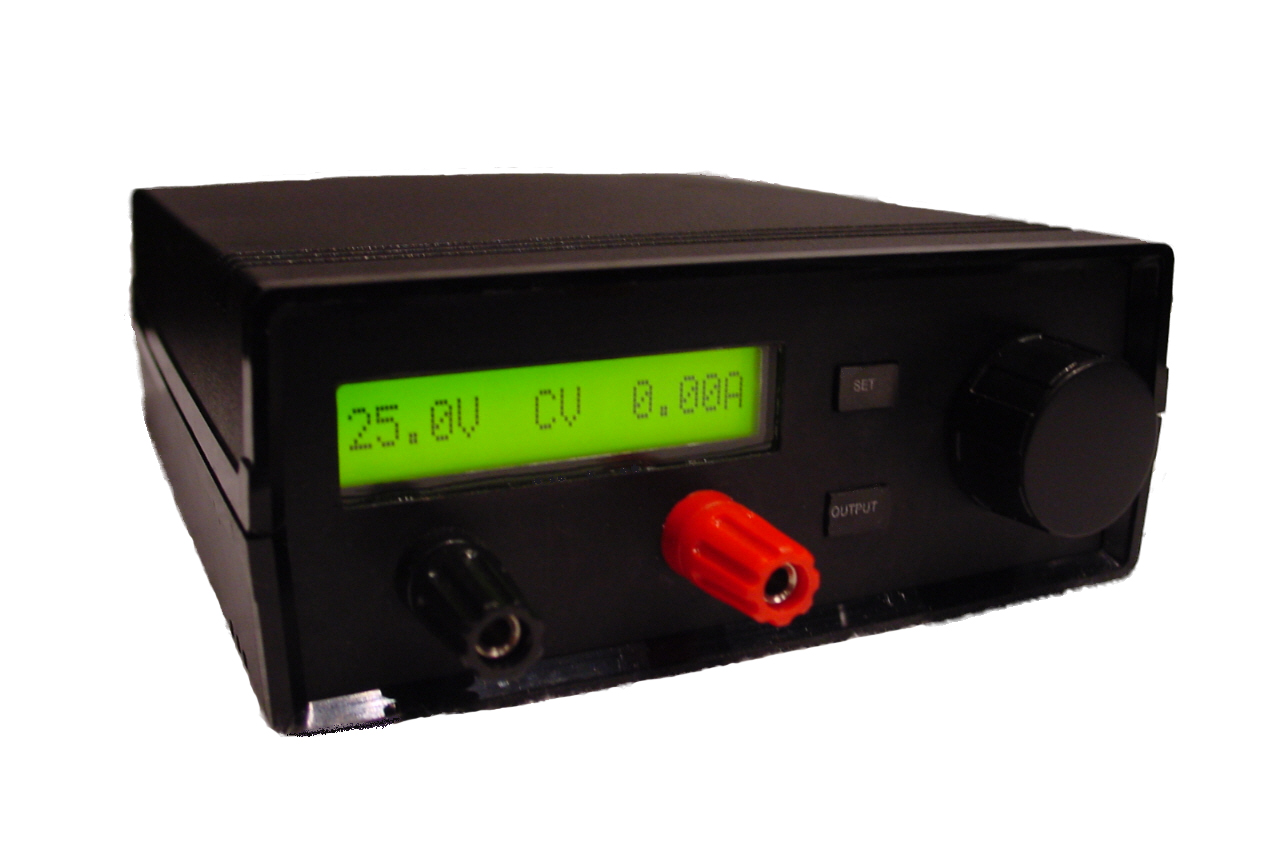
\includegraphics[%
  scale=0.7]{pics/edited/ekstern_copy.jpg}}


\author{Microcontroller Based Laboratory Power supply}

\maketitle
\vspace*{\fill}
Written with \LyX{} in April - May 2004 by Thomas Strand.

\tableofcontents{}


\chapter{Introduction}

\begin{flushleft}Any engineer, technician or hobbyist need some form
of power supply when designing or experimenting with electronic circuits.
The power supply described here will cover a broad range of applications,
including battery charging. AVRpsu is a laboratory power supply with
a single output of 0-25V, 0-2.5A. Output voltage and current limit
are adjustable from the front panel controls or remotely through the
RS-232 port, with resolutions of 100mV and 10mA. The design is entirely
linear, resulting in lower noise than switched designs. A very compact
size is achieved through use of a highly integrated microcontroller,
the Atmel ATmega8. It eliminates the need for external devices such
as A/D- and D/A-converters, memories, clock circuits or any adress
''glue logic''. This saves on design time, cost and space.%
\begin{figure}[h]
\begin{center}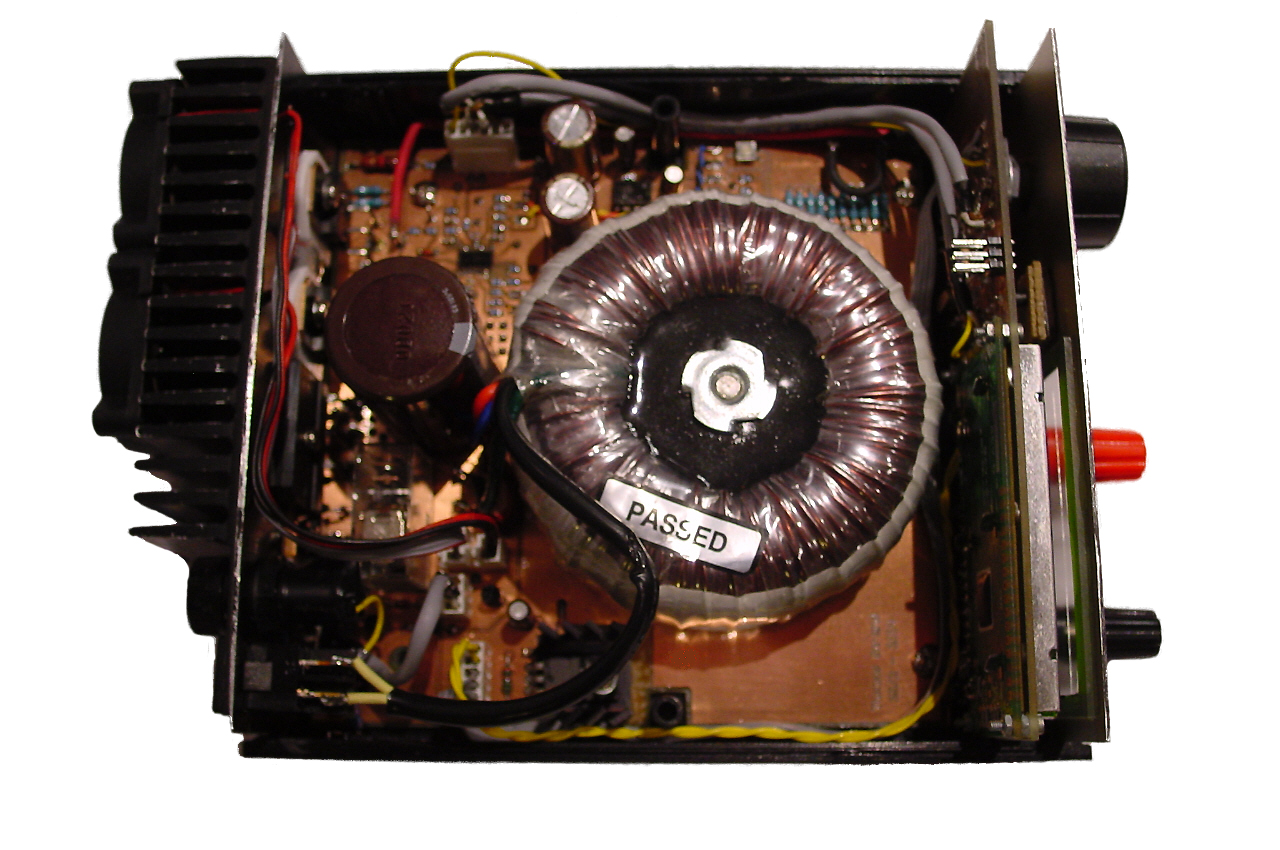
\includegraphics[%
  scale=0.6]{pics/edited/intern_copy.jpg}\end{center}
\end{figure}
\end{flushleft}


\chapter{Operation}


\section{Overview}

AVRpsu may be operated either from the RS-232 port or from the front
panel. The front panel consists of an alphanumeric display, two buttons,
a rotary encoder and a pair of output terminals. The two buttons are
labeled SET and OUTPUT, and are used for selecting which parameter
to adjust and switching the output on or off, respectively. A rotary
encoder is used for adjusting parameters. This simple scheme makes
operation intuitive, eliminating the need for an in-depth study of
the manual before using the unit.

The OUTPUT key is very convenient for switching off the power while
doing modifications to the project at work.

Pressing and holding either of the buttons has special functions.

For operation from the RS-232 port, see section \ref{sec:RS-232-Port}.


\newpage
\section{Adjusting Parameters}

Parameters are adjusted from a set of menus, which are entered by
pressing/holding the keys. The menu structure is illustrated in Figure
\ref{fig:menu} and is explained in detail in the following sections.

%
\begin{figure}[h]
\begin{center}\includegraphics[%
  scale=0.2]{figures/Flowchart.gif}\end{center}


\caption{\label{fig:menu}AVRpsu menu structure.}
\end{figure}



\subsection{Adjusting Voltage and Current}

From \emph{Normal} mode, a short press on SET will enter the \emph{Set
Volt} mode. Every succeeding short press will advance to the next
mode in the list.

\begin{lyxlist}{MMMMMMM}
\item [\emph{Set~Volt:}]Voltage digits are flashing and the voltage setpoint
can be adjusted with the rotary encoder.


If no adjustement is made for about 20 seconds, AVRpsu returns to
\emph{Normal} mode, leaving parameters in EEPROM unchanged. This is
true even if parameters are adjusted from the RS-232 port.

\item [\emph{Set~Ampere:}]Ampere digits are flashing and the current limit
can be adjusted with the rotary encoder.


If no adjustement is made for about 20 seconds, AVRpsu returns to
\emph{Normal} mode, leaving parameters in EEPROM unchanged. This is
true even if parameters are adjusted from the RS-232 port.

\item [\emph{Normal:}]Return to \emph{Normal} mode. The voltage and current
setpoints are saved to EEPROM, and the cycle is repeated.
\end{lyxlist}

\subsection{Switching the Output On or Off}

The output can be toggled on or off with a short press on OUTPUT in
any of the modes \emph{Normal, Set Volt} or \emph{Set Ampere}. When
the output is off, ''OFF'' appears in the output mode field of the
display (see section \ref{sec:out_mode}).


\subsection{Adjusting Baudrate and Fan trip points}

From \emph{Normal} mode, press and hold SET to enter the \emph{Set
Baudrate} mode. Every succeeding short press will advance to the next
mode in the list.

To exit to \emph{Normal} mode again, press and hold SET. The Baudrate
and the Fan trip points are saved to EEPROM.

\begin{lyxlist}{MMMMMMM}
\item [\emph{Set~Baudrate:}]The Baudrate is flashing and can be adjusted
with the rotary encoder. 


Ten Baudrates are available: 300, 600, 1200, 2400, 4800, 9600, 19200,
38400, 57600 and 115200 bps.

The frame format is fixed to 8 data bits, no parity and one stop bit.

If no adjustement is made for about 20 seconds, AVRpsu returns to
\emph{Normal} mode, leaving parameters in EEPROM unchanged. This is
true even if parameters are adjusted from the RS-232 port.

\item [\emph{Set~Fan~Start:}]The Fan Start Temperature is flashing and
can be adjusted with the rotary encoder.


It can be adjusted in the following range: $Fan\, Stop+1\Longrightarrow80$

If no adjustement is made for about 20 seconds, AVRpsu returns to
\emph{Normal} mode, leaving parameters in EEPROM unchanged. This is
true even if parameters are adjusted from the RS-232 port.

\item [\emph{Set~Fan~Stop:}]The Fan Stop Temperature is flashing and
can be adjusted with the rotary encoder.


It can be adjusted in the following range: $30\Longrightarrow Fan\, Start-1$

If no adjustement is made for about 20 seconds, AVRpsu returns to
\emph{Normal} mode, leaving parameters in EEPROM unchanged. This is
true even if parameters are adjusted from the RS-232 port.

\item [\emph{Set~Baudrate:}]Return to \emph{Set Baudrate} mode, and the
cycle is repeated.
\end{lyxlist}

\newpage
\subsection{Viewing Output Power and Heatsink Temperature}

This mode enables the user to see the power consumption of the load
and the measured temperature at the heatsink.

\emph{View Power} mode is entered by pressing and holding OUTPUT.
The power delivered to the load and the heatsink temperature are displayed.
Please note the following:

\begin{itemize}
\item This mode can only be entered from \emph{Normal} mode.
\item No parameters can be adjusted in this mode.
\item Short presses on OUTPUT have no effect in this mode, implying the
output can not be switched on or off in this mode.
\end{itemize}
To exit to \emph{Normal} mode, press and hold OUTPUT.


\subsection{Display}

\begin{floatingfigure}{0.50\columnwidth}%
\begin{center}\includegraphics[%
  scale=0.15]{figures/ModeTable.gif}\end{center}


\caption{\label{fig:display}Display modes.}\end{floatingfigure}%


The display is a LED backlit, 16 characters $\times$1 line alphanumeric
LCD module (Seiko L1671B1J). It has a built-in ASCII translator table,
and eight user-definable characters.

The alphanumeric format is more flexible than traditional seven-segment
types, allowing all sorts of text and icons to be displayed. This
makes menu-based configuration easier to implement, and simplifies
adding features.

Different parameters are displayed according to the selected mode,
as shown in Figure \ref{fig:display}.

Flashing parameters can be adjusted by turning the rotary encoder.
Adjusting a parameter will cause the flashing to stop for a few seconds,
to simplify reading the parameter.

\label{sec:out_mode}In the modes \emph{Normal, Set Volt} and \emph{Set
Ampere}, output mode is shown in the center of the display. output
mode lets the user know whether the voltage or the current is being
regulated (held constant), or if the output has been switched off.
Normally, \emph{Constant Voltage} (CV) is the preferred mode and \emph{Constant
Current} (CC) means the circuit draws more current than expected.
This is, however, not always the case. When charging NiCd batteries,
for example, \emph{Constant Current} is the appropriate mode.

\emph{Output Mode} is one of the following:

\begin{lyxlist}{00.00.0000}
\item [CV]Constant Voltage
\item [CC]Constant Current
\item [OFF]Output has been switched off
\end{lyxlist}

\section{Parameter Storage}

All parameters are saved in non-volatile memory (EEPROM) and restored
at power-up. This makes it convenient to continue working after the
power has been switched off, eliminating the need for re-adjusting
parameters. One exception is the output state, which is always off
at power-up, to prevent accidental destruction of connected equipment.

Parameters are saved on two occasions:

\begin{itemize}
\item When in \emph{Set Ampere} mode and pressing SET for a short time.
AVRpsu will return to \emph{Normal} mode and voltage and current limit
setpoints are saved to EEPROM.
\item When in \emph{Set Baudrate, Set Fan} Start or Set \emph{Fan Stop}
mode and pressing and holding SET. AVRpsu will return \emph{to Normal}
mode and Baudrate and Fan trip points are saved to EEPROM.
\end{itemize}
Parameters received through the RS-232 port will not overwrite those
stored in EEPROM.


\section{\label{sec:RS-232-Port}RS-232 Port}

The RS-232 port can be used for remote control of the AVRpsu, including
readback of measured values. The port is always activated and will
always respond to received commands. The available commands are shown
in table \ref{tab:RS-232}.

%
\begin{table}[h]

\caption{\label{tab:RS-232}RS-232 port commands}

\begin{center}\begin{tabular}{|l|c|c|c|c|}
\hline 
\multirow{2}{10mm}{Command}&
\multicolumn{2}{l|}{Host writes}&
\multicolumn{2}{c|}{Host reads}\tabularnewline
\cline{2-3} \cline{4-5} 
&
ID&
Data&
Data&
\tabularnewline
\hline
\hline 
Set Volt&
''V''&
dd&
&
13d\tabularnewline
\hline 
Set Ampere&
''A''&
dd&
&
13d\tabularnewline
\hline 
Read Volt&
''v''&
&
dd&
\tabularnewline
\hline 
Read Ampere&
''a''&
&
dd&
\tabularnewline
\hline 
Read Temperature&
''t''&
&
dd&
\tabularnewline
\hline 
Output on&
''O''&
&
&
13d\tabularnewline
\hline 
Output off&
''o''&
&
&
13d\tabularnewline
\hline 
Read Output State&
''s''&
&
dd&
\tabularnewline
\hline
\end{tabular}\end{center}
\end{table}


Unsupported commands are replied with a \char`\"{}?\char`\"{}. 

Data values \char`\"{}dd\char`\"{} for different parameters are as
follows:

\begin{lyxlist}{MMMMMMMM}
\item [Voltage:]Decimal numbers in the range 0 - 250 representing 0 - 25.0V.
This applies for both reading and writing, and illegal values are
ignored and replied with a \char`\"{}?\char`\"{}.
\item [Ampere:]Decimal numbers in the range 0 - 250 representing 0 - 2.50A.
This applies for both reading and writing, and illegal values are
ignored and replied with a \char`\"{}?\char`\"{}.
\item [Temperature:]Decimal numbers in the range 0 - 255 representing 0
- 127.5 degrees C. The LSB of the data byte represents 0.5 degrees
and the remaining seven bits represents 0 - 127 degrees C.
\item [Output~State:]One of the following characters:

\begin{lyxlist}{00.00.0000}
\item ['O':]Off
\item ['V':]Constant Voltage (CV)
\item ['C':]Constant Current (CC)
\end{lyxlist}
\end{lyxlist}
When a parameter has been set from the RS-232 port, an icon is shown
in the display, at the left side of the \emph{}output mode field.
This indicates one or more parameters has been altered since the last
setting from the front panel. The icon will be cleared when a parameter
is adjusted from the front panel.


\section{\label{sec:Firmware-Upgrade}Firmware Upgrade}

The internal firmware of the AVRpsu can be upgraded through the RS-232
port. This is possible due to the boot loader support of the Atmega8,
a feature enabling it to reprogram its own program memory. 

The program memory (Flash) and EEPROM memories can be read and written
through the RS-232 port, but no provisions are made for reading or
writing Fuse Bits. This is done in order to prevent the user from
rendering AVRpsu unusable by programming a Fuse Bit combination that
do not work. One example of this is selecting a clock configuration
that does not comply with the actual clock in AVRpsu.

Two requirements must be met to be able to upgrade the firmware:

\begin{itemize}
\item Boot Loader Mode must be entered.
\item A PC with programming software must be available.
\end{itemize}
Holding SET while powering up AVRpsu enters Boot Loader Mode. The
display reads \char`\"{}Boot Loader Mode\char`\"{}.

The programming software must be compliant with Atmel Application
Note AVR109. AVRpsu was designed and tested with AVRprog, but other
compatible programs are available and should work, though they are
not tested.

The firmware can now be upgraded with the programming software. The
display will not change during the firmware upgrade. When the upgrade
is finished, power-cycle AVRpsu and it is ready for use with the new
firmware.

It is not possible to damage the Boot Loader by upgrading the firmware,
implying the Boot Loader can not overwrite itself.


\chapter{Technical Description}


\section{Overview}

AVRpsu is a fairly conventional design, with a few exceptions. The
traditional potentiometers for adjusting voltage and current limit
are replaced by a microcontroller, which generates two analogue voltages
in place of the potentiometers. The microcontroller also takes care
of measuring the voltage and current at the output, as well as controlling
the relay in the Raw Power Supply, measuring the temperature at the
heatsink, and controlling the cooling fans. In addition to all this
it provides a RS-232 port, which can be used for remote control of
the unit. Figure \ref{fig:block_diagram} shows the AVRpsu block diagram.

%
\begin{figure}[h]
\begin{center}\includegraphics[%
  scale=0.2]{figures/Block_diagram.gif}\end{center}


\caption{\label{fig:block_diagram}AVRpsu block diagram.}
\end{figure}



\section{Analogue Circuit}

Figure \ref{fig:main_sch} shows the schematic for the main board,
containing all the analogue circuits. It is followed by a detailed
description for each main portion of the circuit.

%
\begin{figure}[h]
\begin{center}\includegraphics[%
  scale=0.21]{figures/main_sch_small.bmp}\end{center}


\caption{\label{fig:main_sch}The main board schematic reveals a straightforward
design.}
\end{figure}



\subsection{Raw Power Supply}

The Raw Power Supply provides the raw DC voltage to the Power Regulator
and consists of a mains transformer (not in schematic), relay (RL1),
rectifier (BR1) and reservoir capacitor (C4). This voltage contains
a fairly large amount of ripple, but the Power Regulator suppresses
this, so there is virtually no ripple voltage at the output. The voltage
is divided in two ranges in order to minimize power dissipation in
the output transistors. A mains transformer with dual 12V secondaries
connected in series provide the two voltage ranges. A relay (RL1)
switches between the two secondary voltages, resulting in 12 or 24V
AC to the rectifier. The relay is in turn controlled by the microcontroller,
operating it according to the measured output voltage.

Power dissipation is limited by the heatsink; the output transistors
are capable of dissipating all power that can be generated under any
condition. Due to this fact, the relay does not switch from 24V to
12V immediately when the output voltage drops below the threshold,
but does so after a delay of a few seconds. On the up-going slope,
however, the relay operates immediately, in order to track the setpoint
voltage when the user is increasing the voltage. This procedure ensures
minimum wear and maximum life span to the relay.


\subsection{Power Regulator}

The power regulator is a classic analogue circuit built from operational
amplifiers and transistors. It regulates both voltage and current
at the output terminals to limits set by the user. All regulation
is done in this circuit; the microcontroller is not part of the regulation
loop. The microcontroller only provides the setvalue signals for the
regulator. Scaled signals for measuring output voltage and current
are also provided by the regulator circuit.


\subsubsection{Output Stage}

The output stage consists of Darlington transistors T1 and T2 with
emitter resistors R2 - R4 ensuring equal current distribution. PNP
transistors are selected because they enable the voltage drop to be
minimized. The transistor pair obtains their base current from the
constant current source built from T4, D2, R14, D3, D4 and R9. The
current source draws about 3mA of base current for the output transistors,
which is sufficient to drive them into full conduction. However, op-amps
IC2A and IC2D interfere with the circuit, preventing it from drawing
the full 3mA. The op-amps thereby form parts of the voltage and current
regulator.

If the output of one or both of these op-amps goes positive, the voltage
at T4's emitter will rise, the base current for T1 and T2 will decrease,
and the output voltage will decrease. This will happen if the output
voltage is higher than the setpoint voltage, or if the output current
is higher than the setpoint current.


\subsubsection{Voltage Regulator}

IC2A compares the actual output voltage, VOLTAGE\_READ, with the setpoint
voltage, VOLTAGE\_SET. If the actual voltage rise above the setpoint,
the output of IC2A will rise, the Emitter of T4 will rise, and the
Base current for the output transistors will decrease, counteracting
the initial voltage rise.

VOLTAGE\_READ is a DC voltage in the range 0 - 5.12V. It is the output
voltage divided by 5, the voltage divider being formed by R12, R15
and R32.

VOLTAGE\_SET is a filtered PWM signal generated by the microcontroller.

The AD-converter signal is labeled VOLTAGE\_READ in Figure \ref{fig:main_sch}
and has its own voltage divider formed by R13, R16 and R31. This is
done in order to prevent erroneous voltage readings under some conditions.
This occurs when the actual voltage is much lower than the setpoint
voltage, because the op-amp will not allow large voltage differences
between its inputs. The voltage at the non-inverting input of IC2A
will then not reflect the output voltage, but will be pulled up by
the inverting input of the op-amp.

The lower end of R32 could have been connected to ground, but that
would have caused the voltage regulator not to compensate for the
voltage drop across the current sense resistor R40 - R49. IC2B ensures
that this voltage drop is compensated for by lowering the lower end
of R32 to a voltage more negative than ground. This fools the voltage
regulator to believe the output voltage is lower than it actually
is. This portion of the circuit is borrowed from a design featured
in the magazine Allt om Elektronik (Swedish version of Elektor).


\subsubsection{Current Regulator}

IC2D compares the actual output current, CURRENT\_READ, with the setpoint
current, CURRENT\_SET. If the actual current rise above the setpoint,
the output of IC2D will rise, the Emitter of T4 will rise, and the
Base current for the output transistors will decrease, counteracting
the initial current rise.

The actual current, CURRENT\_READ, is is simply the voltage across
the 0.1$\Omega$ 6W current sense resistor (R40 - R49) multiplied
by 20. This results in a voltage in the range 0 - 5.12V representing
0 - 2.55A. This signal is also fed to the AD-converter.

The setpoint, CURRENT\_SET, is a DC voltage in the range 0 - 5.12V,
and is a filtered PWM signal generated by the microcontroller.


\subsection{Thermal Management}

A Dallas 18S20 temperature sensor connected to J2 and two fans connected
to J5 provide for thermal management. The temperature sensor is fixed
to the heatsink close to the output transistor pair. It has a 1-wire
digital interface, occupying only one pin on the microcontroller.
The heatsink temperature is monitored continuously and the cooling
fans are controlled according to trip-points defined by the user.

If the heatsink should reach unacceptable temperatures, an over-temperature
mode is entered. In this mode the output is switched off, the fans
are started and a message scrolls through the display telling what
has happened. When the unit has cooled down, normal operating will
be resumed. The output will remain in the off state, however.


\subsection{Auxiliary Circuits}

The rest of the main board schematics consist mainly of voltage regulators
and interconnections. 

IC1 is an adjustable voltage regulator, LM317, which provides the
+5.12V for the digital circuits. This voltage is adjusted by the potentiometer
R8, which thereby set the gain of both voltage and current regulator
loops.

IC3 is a fixed voltage regulator, 7812, which provides +12V for the
relay, fans, op-amps and bias for the output transistors.

IC4 is a voltage converter, which converts the +12V to -12V. Used
for the op-amps.

T3 is the relay driver and T5 is the driver for the fans.

R36 and R39 are the offset adjustment potentiometers for the current
and voltage regulators, respectively.


\section{Digital Circuit}

Figure \ref{fig:display_sch} shows the schematic for the display
board, containing all digital circuitry.

%
\begin{figure}[h]
\begin{center}\includegraphics[%
  scale=0.21]{figures/disp_sch_small.bmp}\end{center}


\caption{\label{fig:display_sch}Display board schematics. Simplicity seems
to be the rule here.}
\end{figure}


R6 is the contrast adjustment potentiometer for the LCD module.

D1 and D2 are LEDs for illuminating the front panel (not implemented
on the prototype).


\subsection{Microcontroller}

IC1 is an Atmel ATmega8 and is the heart of the system, controlling
it all. Thanks to all its integrated peripherals, very few external
components are needed.

Supply decoupling for the microcontroller is provided for by C2 and
C18. C2 is a Murata filter designed to filter supply lines of digital
circuits. It prevents switching noise from the microcontroller from
entering any analogue circuits.

The ISP (In-System Programming) connector was used during development,
for loading the program into the microcontroller. This is necessary
the first time, as no Boot Loader is present when the device is new.
The ISP is also necessary for programming Fuses and for experimenting
with the Boot Loader.


\subsubsection{AD-Converter}

The internal 10-bit AD-converter has its own supply pin, AVCC, which
is connected to the +5V (actually 5.12V) through a LC-filter consisting
of L1 and C1. This arrangement assures clean power to the sensitive
circuitry of the AD-converter. The AD-converter is configured to use
the AVCC as its reference voltage. This implies a 5.12V input at the
active analogue input will result in a full-scale result.

The AD-converter measures the voltage and current at the output, and
displays the values on the display. The signals V\_READ and C\_READ
(see Figure \ref{fig:display_sch}) are fed to the AD-converter through
separate low-pass filters formed by R4, C4, R5 and C5. Only 8 bits
resolution is used in this design, using the eight most significant
bits from the AD-conversion result. The next significant bit is used
for rounding, however. If the next significant bit is set, the result
is rounded up, otherwise not. This method ensures correct rounding
of the result, but the logic behind it can be somewhat difficult to
realize at first. 

Consider the following example: An AD-converter with a range of 0
- 100 is available but only the two most significant digits are used
in the application. The range will then be 0 - 10, ignoring the least
significant (rightmost) digit. The result will then be 01 for all
\char`\"{}real\char`\"{} results in the range 10 - 19. This means
1.9 is rounded down to 1, which is clearly wrong. Now, if the last
digit is taken into account this can be avoided. Rounding the result
up for all values of the last digit equal to or greater than 5, will
correct the result. The same principle is employed in the AD-conversion
routine in AVRpsu.


\subsubsection{PWM}

Timer1 is used in PWM mode for generating the setvalue signals VOLTAGE\_SET
and CURRENT\_SET (see Figure \ref{fig:main_sch}). This timer has
two PWM channels and these signals are fed to the power regulator
through separate RC-filters, resulting in two DC voltages. These voltages
are proportional to the values in their respective Output Compare
Registers, OCR1A and OCR1B. This functionality realizes two DAC's
with the lowest possible pin usage and component count. Since the
signals are generated entirely in hardware, program flow is only affected
when altering the Output Compare Register values.

One drawback is slow response in change of settings, a result of the
time constant in the RC-filters.


\subsubsection{RS-232 Port}

The internal USART together with the external level converter (see
Section \ref{sub:Level-Converter}) provides a RS-232 port, enabling
settings to be adjusted from a computer, and measurements to be fed
to a computer. It is used in the asynchronous mode, as per the RS-232
standard.

The microcontroller's own program can also be updated through the
serial port, see section \ref{sec:Firmware-Upgrade}. This enables
the advanced user to add features to the unit whenever desired.


\subsection{Support Circuits}


\subsubsection{Display}

The display is a Seiko 16X1 LCD module with LED backlight and built-in
controller (Samsung KS0066). The alphanumeric format gives a flexible
means of displaying information, not limiting the displayable information
to just voltage and current but also serial port parameters, temperature
etc. LCD modules like this also cost less than a load of LED digits
and a driver circuit. 

The display module has an 8-bit parallel interface that is connected
to the microcontroller via a 74HC164 shift register (IC2) to save
port pins. The Read/Write signal is permanently connected to ground,
as no reading from the display is necessary. It is common practice
to read the display's Busy Flag after each command, to make sure the
module is ready before sending any data or command. This is, however,
not entirely necessary as long as the timing requirements are met
with good margin.


\subsubsection{Keys}

OUTPUT (S1) and SET (S3) are connected directly to the microcontroller
and enable the user to switch the output on and off as well as entering
menus for adjusting parameters. The microcontroller has selectable
pull-up resistors for each pin, eliminating the need for external
resistors.


\subsubsection{Rotary Encoder}

The Rotary encoder (S2) is connected directly to the microcontroller.
Again, internal pull-up resistors eliminate the need for external
resistors. The encoder has two mechanical switches, which give two
electrical signals. These two signals are 90 degrees offset, providing
direction information. This results in 4 electrical states, which
are sequenced when rotating, the order of sequencing determining the
direction of rotation. These states are stored in a 4-byte table in
program memory and is used for decoding the rotary encoder. One 4-state
cycle corresponds to two mechanical indents and $\frac{1}{12}$ revolution
on the encoder.

Initially the encoder pins are read and the index to the corresponding
table element is stored in a global variable called \emph{rot\_prev}.
Next time around, the pins are read again, the index is found and
compared to the previously stored one. If they match, no rotation
has occurred, and the function returns 0. If they are not equal, two
\emph{if} statements determine which direction the encoder has rotated,
and the function returns -1 or 1.

Not all 4 transactions between states result in a decoded rotation
step because that would result in 2 digital steps per mechanical indent.
This is not desirable; so only two transactions per direction are
selected to result in decoded rotation. This way the increment/decrement
of the parameter matches the mechanical indents of the rotary encoder.

A simpler method is to wait for an edge on one of the signals, and
then check the level at the other signal to determine the direction.
This has one major drawback, however: The program will hang in that
function until the edge is detected. That is not at all acceptable
in all applications.


\subsubsection{\label{sub:Level-Converter}Level Converter}

IC3 is a Maxim MAX202 and provides the level conversion for the RS-232
port. This is an upgrade from the well-known MAX232, requiring just
100nF capacitors for the charge pump voltage converter. It converts
the 0-5V signals at the microcontroller pins to $\pm$12V at the RS-232
port, in both directions.


\chapter{Performance}

\begin{floatingfigure}[p]{0.65\columnwidth}%
\begin{center}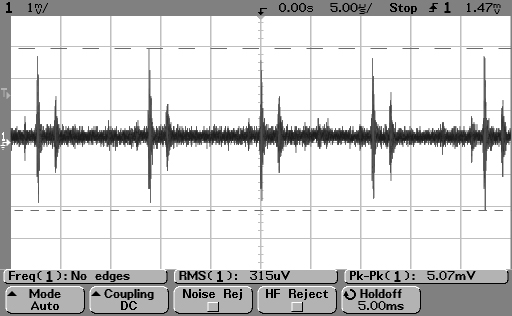
\includegraphics[%
  scale=0.4]{figures/scope_pics/background_noise.jpg}\end{center}


\caption{\label{fig:back_noise}Background noise.}\end{floatingfigure}%


This chapter contains measurements made on the AVRpsu prototype, with
comments. All measurements were made with an Agilent 54622D oscilloscope,
with some supplementing measurements made with a Kenwood CS-5130.
Most measurements were made in a noisy lab, as can be seen on Figure
\ref{fig:back_noise}. This is the resulting scope screen with the
probe tip connected to the ground clip. AVRpsu was set to 25.0V and
2.50A.

All measurements involving low voltages show this noise superimposed
on the output voltage. It is important to realize that this noise
does not arise in the AVRpsu, but rather in the environment where
the measurements were made.


\section{Summary}

\begin{lyxlist}{MMMMMMMMMM}
\item [Noise:]1.5mV$_{\textrm{peak-peak}}$
\item [Ripple~voltage:]4.8mV$_{\textrm{peak-peak}}$max
\item [Ripple~current:]13.6mA$_{\textrm{peak-peak}}$max
\item [Output~resistance:]12.5m$\Omega$
\item [Transient~response:]35$\mu$s
\end{lyxlist}

\newpage
\section{Noise}

\textbf{AVRpsu~settings:} 25.0V 2.50A

Ideally, the output voltage is completely clean under all conditions.
In the real world, however, noise and ripple are superimposed on the
wanted voltage. Noise is measured with no load connected.

Figure \ref{fig:noise} shows the noise on the output voltage with
no load.

\begin{floatingfigure}[p]{0.60\columnwidth}%
\begin{center}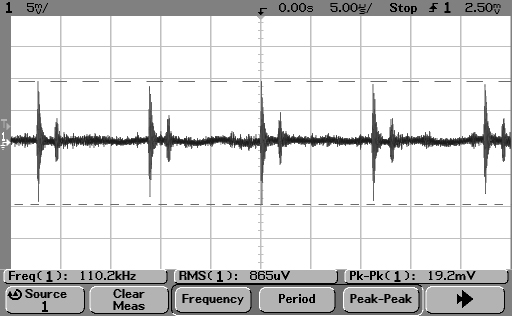
\includegraphics[%
  scale=0.4]{figures/scope_pics/noise_no_load_new.jpg}\end{center}


\caption{\label{fig:noise}Output voltage with noise.}\end{floatingfigure}%


The output voltage resembles Figure \ref{fig:back_noise}, implying
that background noise is very present. If the background noise on
Figure \ref{fig:back_noise} is subtracted, it can be seen that the
AVRpsu noise level is very low.

This measurement was repeated in a different lab, with a Kenwood CS-5130
analogue scope. That revealed about 1.5mV$_{\textrm{pk-pk}}$ of noise
and no spikes around 90kHz.


\section{Ripple}

Ripple is variations in the output voltage and current and is caused
by the varying voltage across the reservoir capacitor. These relatively
large variations arise from the fact that the capacitor is charged
with pulses from the rectifier.


\newpage
\subsection{Ripple Voltage}

\textbf{AVRpsu~settings:} 25.0V 2.50A

Ripple Voltage is measured in Constant Voltage mode, with a load resistor
resulting in a current of 2.49A. Figure \ref{fig:ripple_v} shows
the output voltage under these conditions.

\begin{floatingfigure}[p]{0.65\columnwidth}%
\begin{center}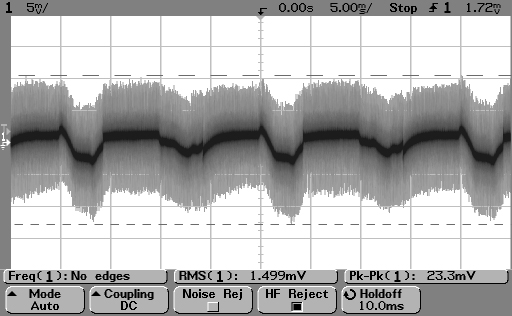
\includegraphics[%
  scale=0.4]{figures/scope_pics/ripple_voltage.jpg}\end{center}


\caption{\label{fig:ripple_v}Ripple voltage.}\end{floatingfigure}%


Noise in the lab is again suspected to be significant. A measurement
made in a different lab with a Kenwood CS-5130 scope indicated a ripple
voltage of 4.8mV$_{\textrm{pk-pk}}$ with very little high-frequency
components. It matched the darkest portion of the trace in Figure
\ref{fig:ripple_v} very well.


\vspace{2cm}
\subsection{Ripple Current}

\textbf{AVRpsu~settings:} 25.0V 2.50A

Ripple Current is measured as a voltage across a load resistor and
calculated using the following formula: $I_{ripple}=\frac{\Delta V}{R_{load}}$

\begin{floatingfigure}[p]{0.65\columnwidth}%
\begin{center}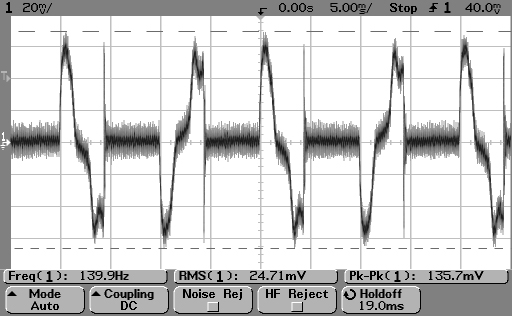
\includegraphics[%
  scale=0.4]{figures/scope_pics/ripple_current_hi.jpg}\end{center}


\caption{\label{fig:ripple_c}Ripple current.}\end{floatingfigure}%


The measurement is performed in Constant Current mode, with a load
resistor resulting in a voltage of 24.9V.

According to Figure \ref{fig:ripple_c}, the ripple current is 2.48mA
RMS. That is less than 0.1\% of the total current, a totally acceptable
figure.


\newpage
\section{Output Switching}

The output voltage does not change instantaneously when pressing the
OUTPUT key. This switching takes time, and the voltage changes in
an exponential slope. The slow response is a result of the method
used for switching the output off: writing zero to the PWM registers.
The delay comes from the low-pass RC-filters for the PWM signals.
This may cause problems when working on digital circuits, as they
tend to dislike slowly rising power supplies.


\subsection{From OFF to ON}

\begin{floatingfigure}{0.60\columnwidth}%
\begin{center}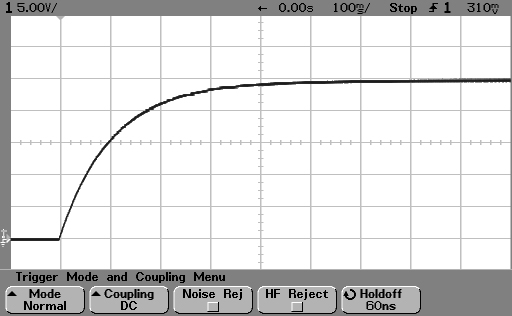
\includegraphics[%
  scale=0.4]{figures/scope_pics/output_off_on.jpg}\end{center}


\caption{\label{fig:off_on}Switching from off to on.}\end{floatingfigure}%


\textbf{AVRpsu~settings:} 25.0V 2.50A

Figure \ref{fig:off_on} shows the output voltage slope when switching
from off to on. The measurement is made with no load.

The slope is slow, but there is no overshoot or any other misbehaviour
at all.


\vspace{2cm}
\subsection{From ON to OFF}

\begin{floatingfigure}[p]{0.60\columnwidth}%
\begin{center}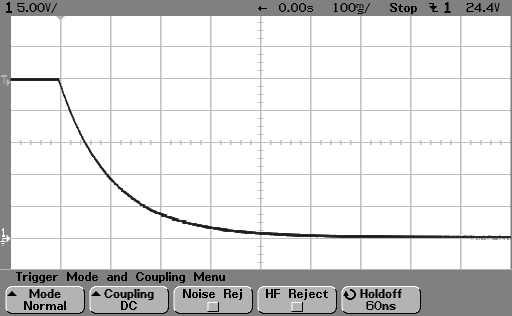
\includegraphics[%
  scale=0.4]{figures/scope_pics/output_on_off.jpg}\end{center}


\caption{\label{fig:on_off}Switching from on to off.}\end{floatingfigure}%


\textbf{AVRpsu~settings:} 25.0V 2.50A

Figure \ref{fig:on_off} shows the output voltage slope when switching
from on to off. The measurement is made with no load.

Again, slow but orderly.


\newpage
\section{Output Resistance}

\textbf{AVRpsu~settings:} 25.0V 2.50A

Output Resistance is defined as the virtual resistance in series with
the output of the power supply. This can be seen by the fact that
the voltage is not constant for different load currents.

The output resistance is measured using the method illustrated in
Figure \ref{fig:rout_setup}. A load resistor is switched on and off
by a function generator and a power FET, causing the load to be stepped
from zero to a known current at a fixed frequency. AVRpsu is in Constant
Voltage mode throughout the measurement.

The output resistance is calculated using the following formula:

\begin{center}$R_{out}=\frac{\Delta V}{\Delta I}$\end{center}

%
\begin{figure}[h]
\begin{center}\includegraphics[%
  scale=0.08]{figures/Rout.gif}\end{center}


\caption{\label{fig:rout_setup}Measuring output resistance.}
\end{figure}


\noindent \begin{flushleft}%
\begin{figure}[h]
\begin{center}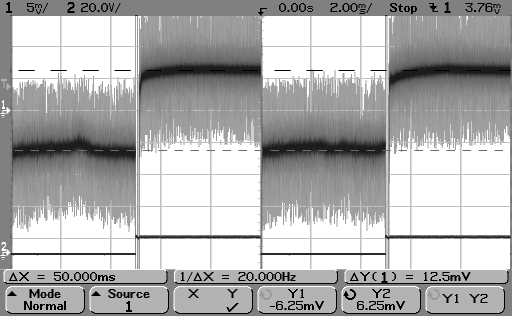
\includegraphics[%
  scale=0.4]{figures/scope_pics/rout.jpg}\end{center}


\caption{\label{fig_rout}Output resistance.}
\end{figure}
\end{flushleft}

The settings and load resistor result in a current of 1.00A, and Figure
\ref{fig_rout} shows a differential voltage of 12.5mV. This equates
to an output resistance of 12.5m$\Omega$, which is a bit on the high
side.


\section{Transient Response}

Transient Response is defined as the time the power supply needs to
get back on track after a change in load.


\subsection{Constant Voltage}

\textbf{AVRpsu~settings:} 10.0V 2.50A

The measurement setup is the same as for output resistance measurement,
see Figure \ref{fig:rout_setup}. The only difference is the oscilloscope
settings regarding timebase and vertical amplifier.

%
\begin{figure}[h]
\begin{center}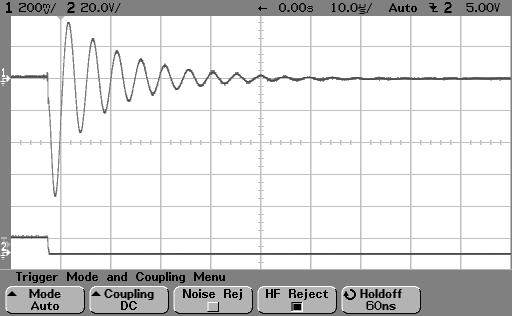
\includegraphics[%
  scale=0.4]{figures/scope_pics/transient_cv.jpg}\end{center}


\caption{\label{fig:trans_cv}Transient response.}
\end{figure}


Figure \ref{fig:trans_cv} shows the measured response, Channel 1
trace is the output voltage, AC coupled. The negative edge on the
Channel 2 trace indicates the load being switched on. The load current
then steps from zero to 1.00A. The Transient Response time is about
35$\mu$s.


\newpage
\subsection{Constant Current}

\textbf{AVRpsu~settings:} 10.0V 0.75A

In Constant Current mode, one resistor is permanently connected to
the output, while another is switched on and off with a power FET,
see Figure \ref{fig:trans_cc_setup}. This way, the output current
is changed from one level to another at a fixed frequency. AVRpsu
is in Constant Current mode during both these phases.

%
\begin{figure}[h]
\begin{center}\includegraphics[%
  scale=0.08]{figures/transient_cc.gif}\end{center}


\caption{\label{fig:trans_cc_setup}Measuring transient response in Constant
Current mode.}
\end{figure}


%
\begin{figure}[h]
\begin{center}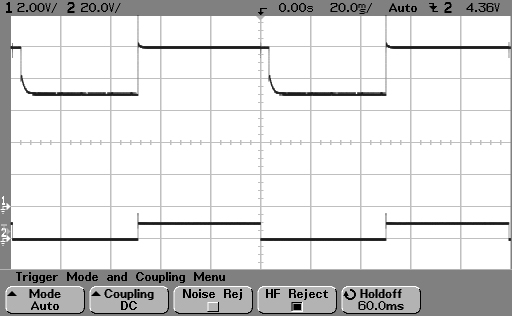
\includegraphics[%
  scale=0.4]{figures/scope_pics/transient_cc_overview.jpg}\end{center}


\caption{\label{fig:trans_cc_over}Transient response overview.}
\end{figure}


Figure \ref{fig:trans_cc_over} gives an overview of what is going
on. Channel 2 represents the extra load resistor being switched on
and off (low is on), while channel 1 shows the output voltage change,
keeping the total current constant.

%
\begin{figure}[h]
\begin{center}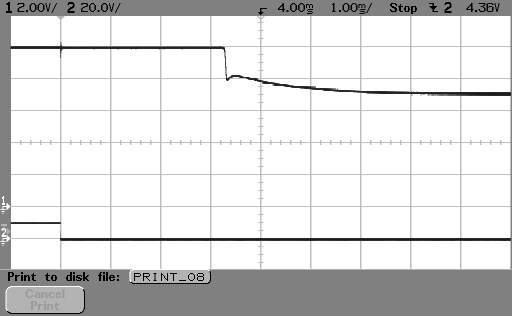
\includegraphics[%
  scale=0.4]{figures/scope_pics/transient_cc_negedge.jpg}\end{center}


\caption{\label{fig:trans_cc_neg}Transient response negative edge detail.}
\end{figure}


\newpage
Figure \ref{fig:trans_cc_neg} shows the details of the output slope
when the current changes from a low level to a high level. This is
the most interesting case, as it represents AVRpsu preventing the
load current from growing larger than the user-defined level.

AVRpsu's current regulator is slow. When the load resistance suddenly
decreases, AVRpsu does not do anything for about 3.3ms, and then it
uses about 3ms to get back on track.

\appendix

\chapter{Circuit Board Layouts}


\section{Main Board}

%
\begin{figure}[h]
\begin{center}\includegraphics[%
  scale=0.2]{figures/main_place_small.bmp}\end{center}


\caption{Main board component placement.}
\end{figure}


%
\begin{figure}[h]
\begin{center}\includegraphics[%
  scale=0.5]{figures/main_top_small.bmp}\end{center}


\caption{Main board top layer.}
\end{figure}


%
\begin{figure}[h]
\begin{center}\includegraphics[%
  scale=0.5]{figures/main_bot_small.bmp}\end{center}


\caption{Main board bottom layer.}
\end{figure}



\section{Display Board}

%
\begin{figure}[h]
\begin{center}\includegraphics[%
  scale=0.2]{figures/disp_place_top_small.bmp}\end{center}


\caption{Display board top layer component placement. Front view.}
\end{figure}


%
\begin{figure}[th]
\begin{center}\includegraphics[%
  scale=0.2]{figures/disp_place_bot_small.bmp}\end{center}


\caption{Display board bottom layer component placement. Front view.}
\end{figure}


%
\begin{figure}[h]
\begin{center}\includegraphics[%
  scale=0.5]{figures/disp_top_small.bmp}\end{center}


\caption{Display board top layer. Front view.}
\end{figure}


%
\begin{figure}[h]
\begin{center}\includegraphics[%
  scale=0.5]{figures/disp_bot_small.bmp}\end{center}


\caption{Display board bottom layer. Front view.}
\end{figure}

\end{document}
